\section{Design}

% Operations
\yifei{feels a bit redundant as we just defined this in the previous
section but we need something to introduce when to use different symbols}

{\color{red}An operation is defined as a tuple containing proc (the
  process that issued the operation, used for session identification),
  type (the type of the operation such as read, write, or custom), obj
  (the object the operation is performed on), ival (operation input
  value), oval (operation output value), stime (invocation time of the
  operation), and rtime (response time of the operation). An operation
  can be conceptualized as a request-response pair, where the request
  is the operation itself and the response is the operation with the
  response time set. Operations do not contain the node that issued or
  handled the operation; they are defined as generic entities that can
  be issued by any node and handled by any node. To add constraints on
  the nodes that can issue or handle an operation, the framework user
must define nodes and edges.}

When modeling multiple interacting systems or components within a
single analysis context, using distinct symbols for the operations
belonging to each system is crucial. Consistency semantics are
typically defined using universally quantified formulas (e.g.,
$\forall a, b: \dots$) applied to relations treated as uninterpreted
functions by the SMT solver (e.g., $\text{vis}(a, b)$,
$\text{so}(a, b)$). If the same symbolic operations (like $a, b$)
and relation functions (like $\text{vis}$) were reused across the
models of different systems within the same solver query, the solver
would treat them as the same entities. This could lead to
unintended interactions and logical conflicts: constraints from one
system's model might implicitly and incorrectly restrict the behavior
of operations logically belonging to another system. By assigning
unique symbols to operations (and potentially relations) associated
with different components (e.g., $a_X$, $b_X$, $\text{vis}_X$ for
System X; $a_Y$, $b_Y$, $\text{vis}_Y$ for System Y), we maintain
the necessary logical isolation. This ensures that the axioms and
constraints of a specific consistency model only apply to the
operations within that specific system's scope. This symbolic
separation is fundamental for enabling the analysis of
cross-system interactions, where specific ``glue''
constraints can then be added explicitly to relate operations across
these distinct symbolic domains, as demonstrated in our cross-service causal
consistency modeling.

% NOTE: from readme
%
% these are more relevant to composition, add them here won't make much sense?
%
% Operation: an operation is defined as a tuple of (from
% non-transactional survey):
% proc: the process that issued the operation (used for session
% identification, e.g. same session constraint).
% type: the type of the operation (e.g. read, write. or custom).
% obj: the object the operation is performed on (e.g. a key in a
% key-value store).
% ival: operation input value (e.g. the value to be written, not used
% anywhere yet).
% oval: operation output value (e.g. the value read, not used anywhere yet).
% stime: invocation time of the operation (i.e. the time the
% operation was issued).
% rtime: response time of the operation (i.e. the time the operation
% was completed).
% Think of an operation as a request-response pair, where the request
% is the operation itself and the response is the operation itself
% with the response time set (assuming the delays between the request
% and the response are equal for all operations, the request takes
% (rtime - stime)/2 time to be sent to the handling node and to be
% processed, vice versa for the response).
%
% (Our own interpretation)
% Operation does not contain the node that issued the operation, nor
% the node that handled the operation. It's defined as a generic
% entity that can be issued by any node and handled by any node. To
% add constraints on the nodes that can issue or handle an operation,
% the framework user must define nodes and edges.

%
% Relation predicates:
% A set of predicates that define the relations between operations in
% a history (also includes those in AE).
% The predicates are used as base/premise for consistency models
% (implementations in relation.py, history.py,
% abstract_execution.py). In the implementation, the predicates are
% singletons and will be added ad-hoc if any clause refers to them.
%

Similar to how Lamport et al. \cite{lamport1977proving} defines
axioms, they are pairwise constraints defined over operations. In
our implementation, these axioms, invariants, and relations are
declared as uninterpreted functions, where the SMT solvers are free
to interpret them so long as they satisfy the imposed constraints.
{\color{red}Relation predicates define the relations between
  operations in a history and are used as base premises for consistency
  models. In the implementation, the predicates are singletons and will
be added ad-hoc if any clause refers to them.}

%
% History (in the actual writing, layout the actual Z3 clauses used
% to encode the relational constraints): a set of operations.
% Add relations between operations within history (returns before,
% same session, session order).
%

A history is a set of operations that have been executed in the
system the tool is modeling \cite{viotti2016consistency}. Although it
is not specifically defined as such in our framework, relations are
quantified over operations to capture the deterministic
orderings of themselves and other operations in the history. The
operations being quantified over form the history, which is
conceptually identical to the set of operations that have been
executed in the system.

Axioms defined for operations within a history include
returns-before: $\text{rb} \triangleq \{(a, b) : a, b \in H
\wedge a.\text{rtime} < b.\text{stime}\}$,
same-session: $\text{ss} \triangleq \{(a, b) : a, b \in H \wedge
a.\text{proc} = b.\text{proc}\}$, session-order:
$\text{so} \triangleq \text{rb} \cap \text{ss}$, and
same-object: $\text{ob} \triangleq \{(a, b) : a, b \in H \wedge
a.\text{obj} = b.\text{obj}\}$.

In our implementation, each history relation function (e.g.,
\texttt{History.Relation.returns\_before}) accepts an optional
\texttt{symbols} argument. This parameter allows framework users to
explicitly specify the symbolic operations (e.g., \texttt{["a\_X",
"b\_X"]}) over which the relation's constraints should be quantified
for that specific instance. This mechanism enables the application of
history-based constraints distinctly to operations belonging to
different modeled systems or components, contributing to the logical
isolation necessary for cross-system analysis. If the
\texttt{symbols} argument is omitted, the functions default to a
standard set of symbols (like \texttt{["a", "b"]}), applying the
constraints to a general set of operations suitable for single-system analysis.

\subsection{Abstract Execution}

%
% Abstract execution (in the actual writing, layout the actual Z3
% clauses used to
% encode the relational constraints): one or more "instantiation" of history. An
% abstract execution is a set of operations (i.e. history) that are further
% constrained by the nondeterminism of the asynchronous environment
% (e.g., message
% delivery order), and implementation-specific constraints (e.g., conflict
% resolution policies) (from non-transactional survey).
%

An abstract execution instantiates and refines the history by
specifying which operations are visible to, or are arbitrated over
each other. Abstract execution relations are non-deterministic
orderings used to capture more complex temporal constraints and
conflict resolution such as visibility, arbitration, and
happens-before relationships. These relations provide the foundation
for modeling sophisticated consistency guarantees that go beyond
simple temporal ordering, enabling the specification of complex
distributed system behaviors where operations may be reordered,
delayed, or selectively visible across different system components.
In other words, multiple abstract executions are possible for a
single history as observed event orderings can differ between nodes.
AE encode the non-deterministic effects of asynchronous execution
environments and implementation-specific constraints
\cite{burckhardt2014principles} \cite{viotti2016consistency}.

Similar to History relations, the Abstract Execution relation
functions in our implementation (e.g.,
\texttt{AbstractExecution.Relation.visibility}) also accept an
optional \texttt{symbols} argument. This allows framework users to
instantiate AE relations with constraints quantified over specific
symbolic operations relevant to a particular system or component
being modeled. Omitting the argument applies the relation to the
default set of symbols.

One of our main contributions is clearly defining
visibility, as existing definitions in the literature are ambiguous
regarding exact behavior under concurrent
settings
\cite{viotti2016consistency,viotti2016towards,zhang2018building,ferreira2023antipode}.
In our implementation, we restructure visibility as a binary relation
and perform explicit case analysis on all possible combinations of
read and write operations that can be "visible" to each other.

We introduce the notion of can-view and viewed to capture the
deterministic and non-deterministic behavior of operations,
and what it means for one operation to be able to "observe"
the effects of another operation. To achieve visibility, two
operations must first fall in one of
the categories in "can-view": either the write happened before the read
in absolute time (note that whether the read/write happened on the
  same process does not matter, as synchronization
is not required to establish probable effect causality)
or the read and write happened concurrently such that the read might
observe the write's effect.

The can-view non-deterministic relation is defined over the pairwise
start or return time between
specified read and write operations. When two operations $a$ and $b$
are defined to be in can-view relation ($a \xrightarrow{\text{can-view}} b$),
either $a$ returned before $b$, such that $b$'s write effect can be
visible to $a$, or $a$ and $b$ happened concurrently such that
$b$'s write effect might be visible to $a$. Formally:

\begin{align*}
  \text{can-view} &\triangleq \{(a, b) : a \in H_\text{rd}, b \in
    H_\text{wr} \land a.\text{obj} = b.\text{obj} \\
    &\land ((
      a.\text{stime} > b.\text{rtime}) \\
      &\lor
      (a.\text{stime} \leq b.\text{stime} \land
        a.\text{stime} \leq b.\text{rtime} \land \\
        &\quad\ \ a.\text{rtime} \geq b.\text{stime} \land
      a.\text{rtime} \geq b.\text{rtime}) \\
      &\lor
      (a.\text{stime} \geq b.\text{stime} \land
        a.\text{stime} \leq b.\text{rtime} \land \\
        &\quad\ \ a.\text{rtime} \geq b.\text{stime} \land
      a.\text{rtime} \geq b.\text{rtime}) \\
      &\lor
      (a.\text{stime} \leq b.\text{stime} \land
        a.\text{stime} \leq b.\text{rtime} \land \\
        &\quad\ \ a.\text{rtime} \geq b.\text{stime} \land
      a.\text{rtime} \leq b.\text{rtime}) \\
      &\lor
      (a.\text{stime} \geq b.\text{stime} \land
        a.\text{stime} \leq b.\text{rtime} \land \\
        &\quad\ \ a.\text{rtime} \geq b.\text{stime} \land
        a.\text{rtime} \leq b.\text{rtime}
      )
  )\}
\end{align*}

The can-view relation is a non-deterministic pairwise
partial ordering that depends solely on timestamps. Conceptually, it captures
all cases where reads happened before, after, or during writes.
It is a set
of operation pairs where the first element is a read and the second
element is a write. The read \textit{can view} the write if (see
Figure \ref{fig:can-view}):

\begin{itemize}
  \item ($a \xrightarrow{\text{can-view}} b_1$) The read-write pair
    does not overlap, thus non-concurrent.

  \item ($a \xrightarrow{\text{can-view}} b_2$) The read started
    before the write starts and ended after the write ends, i.e. the
    write is fully contained within the read.

  \item ($a \xrightarrow{\text{can-view}} b_3$) The read started
    after the write starts and ended after the write ends, i.e. read
    during the write.

  \item ($a \xrightarrow{\text{can-view}} b_4$) The read started
    before the write starts and ended before the write ends, i.e.
    write during the read.

  \item ($a \xrightarrow{\text{can-view}} b_5$) The read started
    after the write starts and ended before the write ends, i.e. the
    read is fully contained within the write.
\end{itemize}

\begin{figure}[h]
  \centering
  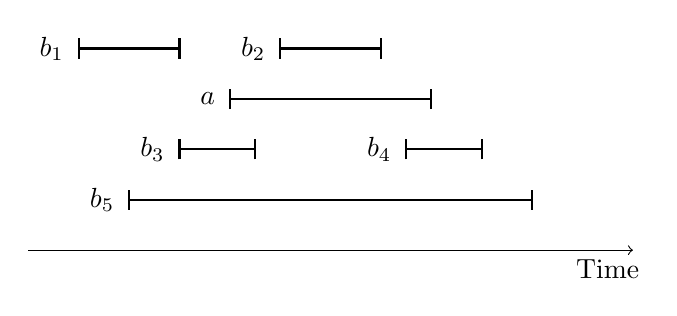
\begin{tikzpicture}[scale=0.64]
    % time
    \draw[->] (0,1) -- (12,1);
    \node[below] at (11.5,1) {Time};

    \draw[thick] (1,5) -- (3,5);
    \draw[thick] (1,4.8) -- (1,5.2); % left terminating bar
    \draw[thick] (3,4.8) -- (3,5.2); % right terminating bar
    \node[left] at (0.9,5) {$b_1$};

    \draw[thick] (5,5) -- (7,5);
    \draw[thick] (5,4.8) -- (5,5.2); % left terminating bar
    \draw[thick] (7,4.8) -- (7,5.2); % right terminating bar
    \node[left] at (4.9,5) {$b_2$};

    % middle
    \draw[thick] (4,4) -- (8,4);
    \draw[thick] (4,3.8) -- (4,4.2);  % left terminating bar
    \draw[thick] (8,3.8) -- (8,4.2);  % right terminating bar
    \node[left] at (3.9,4) {$a$};

    \draw[thick] (3,3) -- (4.5,3);
    \draw[thick] (3,2.8) -- (3,3.2);   % left terminating bar
    \draw[thick] (4.5,2.8) -- (4.5,3.2); % right terminating bar
    \node[left] at (2.9,3) {$b_3$};

    \draw[thick] (7.5,3) -- (9,3);
    \draw[thick] (7.5,2.8) -- (7.5,3.2); % left terminating bar
    \draw[thick] (9,2.8) -- (9,3.2);   % right terminating bar
    \node[left] at (7.4,3) {$b_4$};

    \draw[thick] (2,2) -- (10,2);
    \draw[thick] (2,1.8) -- (2,2.2);   % left terminating bar
    \draw[thick] (10,1.8) -- (10,2.2); % right terminating bar
    \node[left] at (1.9,2) {$b_5$};
  \end{tikzpicture}
  \caption{The can-view relation captures the
    possible visibility between read and write operations. The
    read-write pairs $a_1$, $a_2$, $a_3$, $a_4$, $a_5$ and $b$ are
    defined based on their start and return times, where the read
    operation $b$ can view the effect of the write operation if they fall
  into one of the cases defined in the can-view relation.}
  \label{fig:can-view}
\end{figure}

While can-view captures the possible visibility between read and write, the
result dependency between them is captured by the viewed relation:

\begin{align*}
  \text{viewed} &\triangleq \{(a, b) : a \in H_\text{rd}, b \in H_\text{wr} \\
    &\land (a, b) \in \text{can-view} \\
    &\land (
      (a.\text{oval} = b.\text{ival}) \\
      &\lor
      (\exists x \in H_\text{wr} : (x, b) \in
      \text{can-view} \land a.\text{oval} = x.\text{ival})
    )
  \}
\end{align*}

The viewed relation is defined as a non-deterministic
pairwise partial ordering
between a read and a write that builds upon can-view. Aside from timestamps
falling into one of the can-view cases, we
assign additional value-related
constraints to operations: either the value written by the write
operation must match the output
of the read, or, in case of another write operation
that happened after or
concurrent to the
aforementioned write, the viewed relation enforces the
output of the read to be
from one of the writes (but only one can be chosen). In
the visibility definition, the
transitivity of the viewed relation is implicitly enforced.

Using Figure \ref{fig:can-view}'s operations $a$ and $b_1$ as an example,
since $a$ and $b_1$ are in the can-view relation, if
$b_1$'s written
value matches $a$'s output, then $a$ is in
the viewed relation with $b_1$. Consider
another operation $b_5$ in the same figure that happened
concurrently with $b_1$.
If $b_5$'s written value differs
from $b_1$, but $a$ and $b_5$ are in the can-view
relation and $a$ and
$b_5$ have value
equivalence, then $a$ and $b_1$ are still in the viewed
relation (write
$b_1$ still affects $a$).
However, in this scenario, the constraint in effect for the viewed
relation is the existence of $b_5$ and
the value equivalence of $a$ and $b_5$.

% actual vis
The visibility definition establishes a deterministic pairwise
relationship between any two operations in the history
rather than being
limited to read-write pairs.
It also enforces the transitivity (propagation) and acyclicity
(cannot go back in time) of the viewed
relation. We do not enforce transitivity and acyclicity in the viewed relation
as the orderings of concurrent operations are non-deterministic, and viewed
should include all pairs of operations that can be viewed by each
other based only on logical time and value equality considerations.

When constraint $a \xrightarrow{\text{vis}} b$ is
assigned to a pair
of operations,
the following cases are considered:

% simplest form: can-view -> viewed -> vis + ar
\begin{align*}
  \text{vis} &\triangleq \{(a, b) : \\
    &(a \in H_\text{rd}, b \in H_\text{rd} : \exists x \in
    H_\text{wr}: (x, a) \in \text{vis} \implies (x, b) \in \text{vis}) \\
    &\lor \\
    &(a \in H_\text{rd}, b \in H_\text{wr} : \exists x \in
    H_\text{wr}: (x, a) \in \text{vis} \implies (x, b) \in \text{vis}) \\
    &\lor \\
    &(a \in H_\text{wr}, b \in H_\text{rd} : \text{viewed} \subseteq
    \text{ar}) \\
    &\lor \\
  &(a \in H_\text{wr}, b \in H_\text{wr} : (a, b) \in \text{ar})\}
\end{align*}

Note that the read-read and read-write cases are recursively
defined, where $a$ and $b$ are in $\text{vis}_\text{rd-rd}$ or
$\text{vis}_\text{rd-wr}$, if and only if there exists a
write $x$ that is
visible to $a$, and $x$ is in $\text{vis}_\text{wr-rd}$ or
$\text{vis}_\text{wr-wr}$ with $b$. We call this the
write propagation rule. Conceptually, this means that if a read $a$
and another operation (either read or write) $b$ are in the visibility relation,
the closest write operation $x$ that is visible to read $a$ must
be propagated
to $b$. Whether this visibility relation can be satisfied
depends solely on the existence of read $a$'s previous and
immediately adjacent write operation $x$, and whether
that $x$ can satisfy the write-read or write-write pairwise
constraints of visibility which are
discussed in the following paragraphs.

In the write-read case, we term this rule definitive
visibility. Definitive
visibility is defined as follows: if a write $a$ is
visible to a read $b$, then $b$
must have viewed $a$ and an arbitration relation must exist between $a$ and $b$
to ensure the non-deterministic viewed relation has a
linearization point,
i.e., to cut off one of the possible paths in the viewed relation.

The last case is write-write visibility (write arbitration).
Whether two writes are visible to each other depends on the existence of an
arbitration relation between them. In Viotti et al.
\cite{viotti2016consistency}, the authors clearly stated that two writes
are invisible to each other if not
ordered by vis,
and arbitration imposes a total order to resolve conflicts between concurrent
and invisible operations.

Other relations under Abstract Execution includes arbitration, and
happens-before.
Arbitration is an application specific, transitive and acyclic
relation that provides a total order on conflicting operations,
ensuring that observed executions follow a single coherent timeline. In
our implementation, arbitration is assigned strong timestamp total ordering.
Realistically, arbitration can be achieved with monolithic
sequencers, deterministic
conflict resolution rules, distributed timestamping \cite{lamport1978time},
or consensus protocols
\cite{birman1991lightweight,hadzilacos1994modular,lamport2001paxos}.
Happens-before is used to capture probable causality,
and is previously defined in the literature as the transitive union
of session order and visibility:
$hb \triangleq (\text{so} \cup {\text{vis}})^{+}$
\cite{burckhardt2014principles,viotti2016consistency}.

\subsection{Consistency Semantics}

\subsubsection{Eventual Consistency} ensures that replicas will achieve
identical states when no additional updates occur. Specifically, when
no new write operations are issued, all read operations will
ultimately return the same
value \cite{terry1994session, eventual, viotti2016consistency}. Given
that the liveness
aspects of eventual consistency are characterized through eventual
visibility \cite{viotti2016consistency},
our framework excludes liveness properties and concentrates on safety
properties:
non-circular causality (acyclic projection of the happens-before
relation defined previously) and
contextual return value consistency (a predicate on abstract
  executions ensuring that the return value of any operation within
that execution belongs to the set of its valid return values)
guided under the can-view relation.

\begin{align*}
  &\text{EC}(\mathcal{F}) \triangleq \text{acyclic}(hb) \land \forall
  op \in H: op.oval \in \mathcal{F}(op, ctx(A, op)) \\
  &\text{where} \\
  % for all read op, the ival of operations thats in can-view relation with op
  &\mathcal{F}_{\text{can-view}}(op, ctx(A, op)) = \{x.ival \in
  H_\text{wr} : (op, x) \in \text{can-view}\}
\end{align*}

\subsubsection{Monotonic Reads} guarantees that consecutive read operations
observe a monotonically increasing set
of write effects. When a process observes a particular value $v$ from an object,
subsequent read operations cannot return values from writes that preceded $v$.
This property ensures that read operations can only be satisfied by
replicas that have
applied all write operations previously observed by the
requesting process.

$$
\text{MR} \triangleq \forall a \in H, \forall b, c \in H_\text{rd}: a
\xrightarrow{\text{vis}} b \land b \xrightarrow{\text{so}} c \implies
a \xrightarrow{\text{vis}} c
$$

\subsubsection{Monotonic Writes} guarantees that write operations are
applied to a replica
only after the replica has executed all preceding writes from the same session.
This constraint requires that replicas process all writes within a session
in the exact sequence they were originally issued.

$$
\text{MW} \triangleq \forall a, b \in H_\text{wr}: a
\xrightarrow{\text{so}} b \implies a \xrightarrow{\text{ar}} b
$$

\subsubsection{Read Your Writes} (also read my writes)
mandates that read
operations issued by a process can only be executed by replicas that have
previously applied all writes issued by that same process.

$$
\text{RYW} \triangleq \forall a \in H_\text{wr}, \forall b \in
H_\text{rd}: a \xrightarrow{\text{so}} b \implies a \xrightarrow{\text{vis}} b
$$

\subsubsection{Write Follows Read} or session causality, represents the
inverse principle of the read-your-write guarantee by requiring that
writes performed
within a session are sequenced after any writes from any process on any
object whose effects were observed by preceding reads in the same session.

$$
\text{WFR} \triangleq \forall a, c \in H_\text{wr}, \forall b \in
H_\text{rd}: a \xrightarrow{\text{vis}} b \land b
\xrightarrow{\text{so}} c \implies a \xrightarrow{\text{ar}} c
$$

\subsubsection{Pipeline RAM Consistency} (also PRAM or FIFO
consistency) requires
that all processes observe write
operations from any given process in the identical order as they were
originally issued by
that process. Conversely, processes may witness writes from
distinct processes in varying orders. Therefore, no universal total ordering is
necessary. Nevertheless, writes originating from any single process
(session) must be
ordered sequentially, resembling a pipeline structure.

$$
\text{PRAM} \triangleq \forall a, b \in H: a \xrightarrow{\text{so}}
b \implies a \xrightarrow{\text{vis}} b
$$

\subsubsection{Causal Consistency} surpasses PRAM and
session guarantees in scope. Our causal consistency formulation
combines concepts from Viotti et
al.~\cite{viotti2016consistency}
and causal memory~\cite{baldoni2002an}. The
\textit{writes-into} relation~\cite{baldoni2002an} connects write
operations directly with the reads that retrieve their values. This
guarantees that when
a read operation observes a specific write, all following writes
within the same session
honor that causal sequence. The formalization coordinates session order,
arbitration, visibility, and writes-into to preserve consistent
causal histories.

Operations belong to the \texttt{wi} set when: a write $a$
writes into a read $b$ if and only if $b$ retrieves
the value initially written by $a$, and $a$ and $b$
access the same object (identical memory region). Each $b$ can have at
most one corresponding $a$, maintaining acyclicity.
When one operation succeeds another in session order, their
relationship within the
abstract execution faces additional constraints. Particularly, if $(a, b)
\in \text{so}$,
then $a$ must write-into $b$ when $b$ represents a read operation,
and $a$ must be visible and
arbitrated prior to $b$. Consequently, session order establishes a causal
sequence that manifests
in the relations wi, vis, and ar.

$$
\text{CC} \triangleq \text{WFR} \land \forall a, b \in H: (a, b) \in
\text{so} \implies (a, b) \in \text{wi} \cap \text{vis} \cap \text{ar}
$$

These constraints collectively establish a causal memory model where
session order,
observed values, and write sequences maintain alignment, ensuring
causally dependent writes
manifest in proper order from any observer's viewpoint.

\subsubsection{Liniearizability} is widely considered the gold
standard for strong
consistency In our encoding, we introduced a modified single global
order constraint to unify visibility and
arbitration for all write operations whether for operations in
session-based semantics or not, and tried to enforce real-time ordering to
ensure that the observed histories comply with returns-before relations
(linearization as operations comes in instead of lazily ordering events when
reads occur \cite{zhang2018building}).

\begin{align*}
  &\text{LIN} \triangleq (\forall a, b \in H: [a
    \xrightarrow{\text{vis}} b \implies a \xrightarrow{\text{ar}} b] \\
    &\land [a \xrightarrow{\text{ar}} b \land a.rtime < \infty \implies
  a \xrightarrow{\text{vis}} b]) \\
  &\land rb \subseteq ar \\
  &\land \forall x \in H: x.oval \in \{y.ival \in H_\text{wr} : (x,
  y) \in \text{can-view}\}
\end{align*}
